\documentclass[]{agujournal2019}\usepackage[]{graphicx}\usepackage[]{xcolor}
% maxwidth is the original width if it is less than linewidth
% otherwise use linewidth (to make sure the graphics do not exceed the margin)
\makeatletter
\def\maxwidth{ %
  \ifdim\Gin@nat@width>\linewidth
    \linewidth
  \else
    \Gin@nat@width
  \fi
}
\makeatother

\definecolor{fgcolor}{rgb}{0.345, 0.345, 0.345}
\newcommand{\hlnum}[1]{\textcolor[rgb]{0.686,0.059,0.569}{#1}}%
\newcommand{\hlstr}[1]{\textcolor[rgb]{0.192,0.494,0.8}{#1}}%
\newcommand{\hlcom}[1]{\textcolor[rgb]{0.678,0.584,0.686}{\textit{#1}}}%
\newcommand{\hlopt}[1]{\textcolor[rgb]{0,0,0}{#1}}%
\newcommand{\hlstd}[1]{\textcolor[rgb]{0.345,0.345,0.345}{#1}}%
\newcommand{\hlkwa}[1]{\textcolor[rgb]{0.161,0.373,0.58}{\textbf{#1}}}%
\newcommand{\hlkwb}[1]{\textcolor[rgb]{0.69,0.353,0.396}{#1}}%
\newcommand{\hlkwc}[1]{\textcolor[rgb]{0.333,0.667,0.333}{#1}}%
\newcommand{\hlkwd}[1]{\textcolor[rgb]{0.737,0.353,0.396}{\textbf{#1}}}%
\let\hlipl\hlkwb

\usepackage{framed}
\makeatletter
\newenvironment{kframe}{%
 \def\at@end@of@kframe{}%
 \ifinner\ifhmode%
  \def\at@end@of@kframe{\end{minipage}}%
  \begin{minipage}{\columnwidth}%
 \fi\fi%
 \def\FrameCommand##1{\hskip\@totalleftmargin \hskip-\fboxsep
 \colorbox{shadecolor}{##1}\hskip-\fboxsep
     % There is no \\@totalrightmargin, so:
     \hskip-\linewidth \hskip-\@totalleftmargin \hskip\columnwidth}%
 \MakeFramed {\advance\hsize-\width
   \@totalleftmargin\z@ \linewidth\hsize
   \@setminipage}}%
 {\par\unskip\endMakeFramed%
 \at@end@of@kframe}
\makeatother

\definecolor{shadecolor}{rgb}{.97, .97, .97}
\definecolor{messagecolor}{rgb}{0, 0, 0}
\definecolor{warningcolor}{rgb}{1, 0, 1}
\definecolor{errorcolor}{rgb}{1, 0, 0}
\newenvironment{knitrout}{}{} % an empty environment to be redefined in TeX

\usepackage{alltt}
\usepackage{url} %this package should fix any errors with URLs in refs.
\usepackage{lineno}
\usepackage[inline]{trackchanges} %for better track changes. finalnew option will compile document with changes incorporated.
\usepackage{soul}
\linenumbers



% LTeX: language=en-US

\usepackage{color}
\newcommand*{\todo}[1]{\textbf{\textcolor{red}{(#1)}}}
\newcommand*{\mref}{\todo{ref}}

\usepackage{xr}
\externaldocument[SM-]{../supporting info/supp_info_hail}

% Goes against template but looks a lot nicer.
\justifying 

% Maximum 12 PUs where 1 PU = 500 words or 1 display element (figure or table).
% E.g. 

% To mark revisions:
%
%  \note[editor]{The note}
%  \annote[editor]{Text to annotate}{The note}
%  \add[editor]{Text to add}
%  \remove[editor]{Text to remove}
%  \change[editor]{Text to remove}{Text to add}

\draftfalse
\journalname{Geophysical Research Letters}
\IfFileExists{upquote.sty}{\usepackage{upquote}}{}
\begin{document}

\title{Changes in damaging hail in major Australian cities with global warming}

\authors{Timothy H. Raupach\affil{1,2,3}, Joanna Aldridge\affil{4,5}}

\affiliation{1}{UNSW Institute for Climate Risk and Response, 
                UNSW Sydney, New South Wales, Australia}
\affiliation{2}{UNSW Climate Change Research Centre, 
                UNSW Sydney, New South Wales,  Australia}
\affiliation{3}{ARC Centre of Excellence for Climate Extremes, 
                Sydney, New South Wales,  Australia}
\affiliation{4}{School of Geosciences, University of Sydney, 
                Sydney, New South Wales,  Australia}
\affiliation{5}{QBE Australia, Sydney, 
                New South Wales, Australia}

\correspondingauthor{Timothy H. Raupach}{timothy.h.raupach@gmail.com}

\begin{keypoints}
\item Hail causes more damage when hailstones are larger or coincident winds are stronger, yet uncertainty is high on changes in these factors with global warming.
\item Convection-permitting downscaled simulations were used to investigate possible future changes in hail size and coincident wind strength over major Australian cities and the remote Goldfields region.
\item The projections indicate increases in hailstorm severity in areas around Melbourne, Canberra and Sydney, with increased windblown hail risk in the remote Goldfields region, and non-significant changes in other studied domains.
\end{keypoints}

\begin{abstract} %% 150 words
      In Australia, hailstorms are a leading cause of insured losses, with damage exacerbated if hailstones are large or there are coincident strong winds. Despite the high damage potential of such storms, changes to their frequency and severity under global warming are not well understood. Here, we use downscaled simulations over major cities and a remote region in Australia to project changes in hail frequency, hailstone size, and coincident wind speeds under a future scenario with $\sim$2.8~$^{\circ{}}$~Celsius warming over pre-industrial global mean temperature. The study regions cover over 60\% of the total Australian population. Generalized extreme value analysis was used to examine changes in daily maximum hail sizes and coincident wind speeds. The projections show higher future hail damage potential in some regions, with increases in hail frequency in the Sydney/Canberra and Brisbane regions, and robust increases in maximum hail size and coincident wind strength in the Melbourne and Sydney/Canberra regions.
\end{abstract}

\section*{Plain Language Summary}

Hailstorms endanger lives and damage property, leading to large insured losses in Australia. Hailstorms are more damaging if the hailstones they produce are larger. They are also more damaging if there is high wind at the same time, because the wind can throw hailstones sideways into breakable materials like windows or house facades. We expect climate change to affect hailstorms, but there have been few studies on how hailstorm frequency and severity may change in future in Australia. In this study we used simulations of weather in a future, warmer climate scenario to look at possible changes in hailstone size and in the strength of winds when hail occurs, over major cities and a remote area in Australia. The simulations project an increase in hail severity for the heavily populated Melbourne and Sydney/Canberra regions, an increase in hail frequency in Sydney/Canberra and Brisbane regions, and no significant changes in the other areas we studied.

\section{Introduction}

Severe convective storms are responsible for insured losses of over \$A40b in Australia from 1967 to 2023 (in 2022 dollars), accounting for 25\% of insured catastrophe losses \cite{ICA_2024}. This includes the largest insured loss in Australian history: the April 1999 hailstorm impacting the eastern suburbs of Sydney, at \$8.845b \cite<normalized to 2022 dollars, >{ICA_2024}. Insured losses due to severe convective storms are attributable to several hazards that can occur within the same event: hail, extreme winds, and extreme rainfall. Examination of recent loss history shows that high wind speeds are a common feature of many of the most damaging hailstorms \mref{}. Climate change is expected to affect severe storms \cite{Allen_2018} including hailstorms \cite{Raupach_NREE_2021} and convective winds \cite{Brown_JGRA_2021}. However, a lack of observational data for trend analysis, and the high computational cost of high-resolution modelling, has meant that expected changes in these individual hazards remain highly uncertain \cite{Raupach_NREE_2021,Brown_JGRA_2021}, and changes in the co-occurrence of hail and high winds are virtually unstudied \todo{check}. Here, we use high-resolution downscaled simulations of a future, warmer environment to compare changes in hail damage potential over major population centers of Australia.

\todo{Why consider hail and wind together.} Hail and convective winds are often studied separately. Typical severe convective storm catastrophe models generate synthetic event sets of hail and wind hazards as separate event footprints \mref{}. However, the coincidence of wind and hail is an important driver of loss. Wind-driven hail, both due to its greater force and oblique angle of impact, has greater potential to injure people, destroy crops \cite{Changnon_JAMC_1967, Towery_JAMC_1976} and cause damage to the built environment, such as damaging cladding to external walls, smashing windows of buildings and motor vehicles and letting rainwater inside to damage internal fixtures and contents \mref{}. Examination of recent high-loss hail events in Australia shows that wind is often mentioned as a contributing factor \mref{}.


\todo{What is known about wind driven hail conditions.} Damaging hail is considered to be stones over 2 cm \mref{}. \cite{Allen_2018} writes 90 km/h for severe winds. Wind driven hail events are defined as hail exceeding 5 cm and wind gusts exceeding 100 km/h (27.8 m/s) occurring in the same system within a one-hour timeframe \mref{}. Wind driven hail events are most likely to be associated with supercells where downbursts occur \mref{}. \cite{Carletta_2010} identified that squall lines and isolated cells and clusters of cells as the most frequent systems associated with wind driven hail for the USA using observational data. \cite{Bell_WF_2023} has compiled 1646 hail and wind damage swaths for the mid west of the USA using MODIS satellite observations for use in future understanding of the frequency of these events.

\todo{What is known of hail and wind changes with global warming.} \cite{Allen_JC_2014} used an environment-based approach to suggest an increase in severe thunderstorm incidence in south-east Australia, although with a wide range of uncertainty. \cite{Walsh_CC_2016} review the current and future storm-related wind and hail hazard in Australia and found future projections of wind hazard increase along the populated east coast of Australia. 

\todo{What is the Australian context?} While wind loadings are currently considered in the Australian building code \cite{ABCB_2024} under standard AS1170.2 \cite{Standards_2021}, the impact of hail and wind-driven hail is not currently considered in Australian building design. The \citeA{ACSE_2022} discuss hail loading on roofs and acknowledge that this effect is not accounted for under the current design standards. The April 2015 hail event impacting western Sydney is discussed including the collapse of warehouse buildings from hail loading on roofs. A guide of ultimate limit and service limit state designs for various building types is presented, but wind driven hail is not considered. Some roofing products are tested for hail impacts against standards, but many products are unrated. In ICC building code \cite{ICC_2008}, hail is considered in two hail regions in the USA defined using observational data: moderate and severe, depending on the likelihood of at least one day of 1.5--3 mm \todo{check} hail in a 20-year period. This code requires testing of roofing materials such as asphalt, wood and slate shingle, clay or concrete tiles, metal roofing panels and shingles in these zones. The changing occurrence of hail over time is not considered. In Canada, while hail impact is not considered in the current building code, although change is being sought in the aftermath of the 2020 Calgary hailstorm which caused \$C1.4b of insured loss. Resilience measures may include increasing roof slope, using resistant roofing materials and roof underlays \cite{ICLR_2018}. They found that a steeper roof limits damage from wind-driven hail on the leeward side. The lack of research into impact resistant non-roof housing elements, such as windows, doors, sidings, fascia and skylights, is noted, and these elements are often subject to damage in the most destructive storms.

Here, we seek to understand how the coincidence of extreme winds and damaging hail may change in a future climate in Australia. We considered analyses covering the major Australian cities of Perth, Adelaide, Melbourne, Canberra, Sydney, and Brisbane, and a remote region around the town of Kalgoorlie in the Western Australian Goldfields region. The populations of these cities add to over 60\% of the total Australian population \mref{}. Proxy-based climatologies show these regions to be hail-prone \cite{Raupach_npjCAS_2023}.

\section{Methods}

\subsection{Simulations of historical and projected weather}

Historical and future simulations were produced using the Advanced Research Weather Research and Forecasting (AR-WRF) weather model version 4.4.1 \cite{Skamarock_2021} for six nested domains. Two model configurations were used, with settings other than the domain configurations the same for both (Supporting Information Table \ref{SM-tab:schemes}). In total, we used two coarse- ($\sim$27 km grid spacing), four medium- ($\sim$9 km), and six fine-resolution ($\sim$3 km) domains with a parent-child scaling ratio of three (Supporting Information Figure \ref{SM-fig:domains}). WRF-HAILCAST \cite{Adams-Selin_WF_2019} was enabled for the fine-resolution domains, to estimate maximum hailstone diameters at the surface. Boundary condition inputs were prepared using the \texttt{nc2wrf} code of \citeA{Xu_code_data_2021}. 

Simulations were run for two epochs of 20 convective seasons each: the historical epoch ran from 1989 to 2009, and the future epoch from 2080 to 2100. For each convective season, simulations were run from 00Z September 30 to 18Z February 28, with hourly output resolution. Outputs were converted to local summer time and subset to cover October 1 to February 28 inclusive in each season. For each season the 14 to 16 simulated hours on 30 September local time were discarded as model spin-up time. Model outputs provide instantaneous hourly values for most variables, including wind speed at 10 m. In contrast, for each grid point and each hour, HAILCAST output the maximum hail diameter over all model time steps during the previous hour. The time step for the coarse domain was set to 100 s, but reduced to 80 s or 60 s for simulation days on which Courant-Friedrichs-Lewy (CFL) errors occurred. HAILCAST was run at every model time step, so on those days for which the time step was reduced, HAILCAST ran more often. However, here we use maximum hail sizes per day, and the sample of hail sizes per day is large, so we expect minimal effect of this time step variability. Except for the overall maxima shown in Section \ref{sec:overall_maxima}, we subset all our analyses to consider only times and locations where there was non-zero surface hail recorded in the preceding hour. Wind speeds and convective ingredients are thus instantaneous values in temporal proximity to hail occurrences.

\subsection{Preprocessing of simulation outputs}

Examination of maximum hail size fields showed that HAILCAST occasionally produced unreasonably large hail sizes, particularly over water bodies (Supporting Information Figure \ref{SM-fig:maxes_with_removed_pts}). Since our focus is on hail hazard on land, we subset the data to land areas using the WRF land mask with small holes filled and a slight erosion applied so that points over the ocean, large bodies of water, or directly over the coastal boundary are not considered in this study. Further, we removed from consideration any HAILCAST value of surface hail over 180 mm diameter \cite<this value being greater than the largest hail ever observed in Australia, at $\sim$16 cm,>{BOM_2021}. HAILCAST has been updated in more recent versions of WRF than used here, and while the updated version reduces the occurrence of unrealistically large hail sizes the changes do not affect the majority of HAILCAST results, meaning that removing very large hail sizes as we do here leaves a reasonable dataset for analysis (pers. comm. B. Adams-Selin, 2024). In all, less than 0.006\% of non-zero hail-diameter values (not over water) were removed for being too large, per domain.

\subsection{Statistical modelling of extreme values}

Extreme value analysis was completed using the R \cite{R_software} package \texttt{extRemes} \cite{Gilleland_JSS_2016}. Block maxima were defined as daily maximum hailstone sizes and wind speeds at hail locations per domain, under the assumption that such time series can be considered independent \cite{Coles_2001} because single hail storms do not last more than one day. Generalized extreme value (GEV) distributions were fitted to each series of block maxima. We used quantile-quantile (QQ) plots \cite{Coles_2001} and the Kolmogorov–Smirnoff (KS) test to assess the goodness of fit of the GEV distributions, by examining the similarity of the empirical distributions of block maxima and values drawn from the fitted GEV distributions. The KS test was also used to examine the (dis)similarity of GEV distributions fitted to historical versus future epochs. When the KS test was used, we generated a probabilistic view of the similarity between distributions by drawing 1000 values from the GEV distribution(s), applying the KS test, and repeating this process 100 times to generate 100 KS test results.

\section{Data}

Boundary conditions used for the simulations were bias-corrected data for downscaling by \citeA{Xu_SD_2021}. These boundary conditions have a mean climate and interannual variance derived from European Centre for Medium-Range Weather Forecasts Reanalysis 5 \cite<ERA5,>{Hersbach_QJRMS_2020}, with a non-linear trend derived from the ensemble mean of 18 Coupled Model Intercomparison Project Phase 6 \cite<CMIP6,>{Eyring_GMD_2016} models \cite{Xu_SD_2021}. Future projections used the ``middle-of-the-road'' SSP2-4.5 shared socioeconomic pathway \cite<SSP,>{ONeill_GEC_2017}. On average the historical period in our simulations (1989--2019) had a global mean temperature 0.39 K over pre-industrial temperatures \cite<1850--1990, using the CMIP6 35-model ensemble,>{Gutierrez_2021} while the future period (2080--2099) had a global mean temperature 2.81 K over pre-industrial temperatures. The historical and future epochs were thus separated by 2.42 K of warming.

\section{Results}
\label{sec:results}

\subsection{Overall maxima}
\label{sec:overall_maxima}

Before taking a more rigorous statistical approach, it is useful to consider the maps of overall maxima for the quantities of interest here: hailstone size, and 10 m wind speed at hail hours. Figure \ref{fig:max_hail_sizes_by_domain} shows overall maximum hail sizes across each domain for each epoch. Hailstorm tracks are visible. By eye, an increase in maximum hail sizes is apparent for domains other than Perth and Brisbane, with increases in storm coverage or activity in the Adelaide, Goldfields (Kalgoorlie), Melbourne and Canberra/Sydney domains. Maximum wind speeds at hail hours are more widespread in the future scenarios than the historic scenarios, with an eastward expansion in areas experiencing maximum wind speeds in the Brisbane and Adelaide domains and a southern shift in the Goldfields (Kalgoorlie) region (Supporting Information Figure \ref{SM-fig:max_wind_by_domain}).

\begin{figure}[!h]
      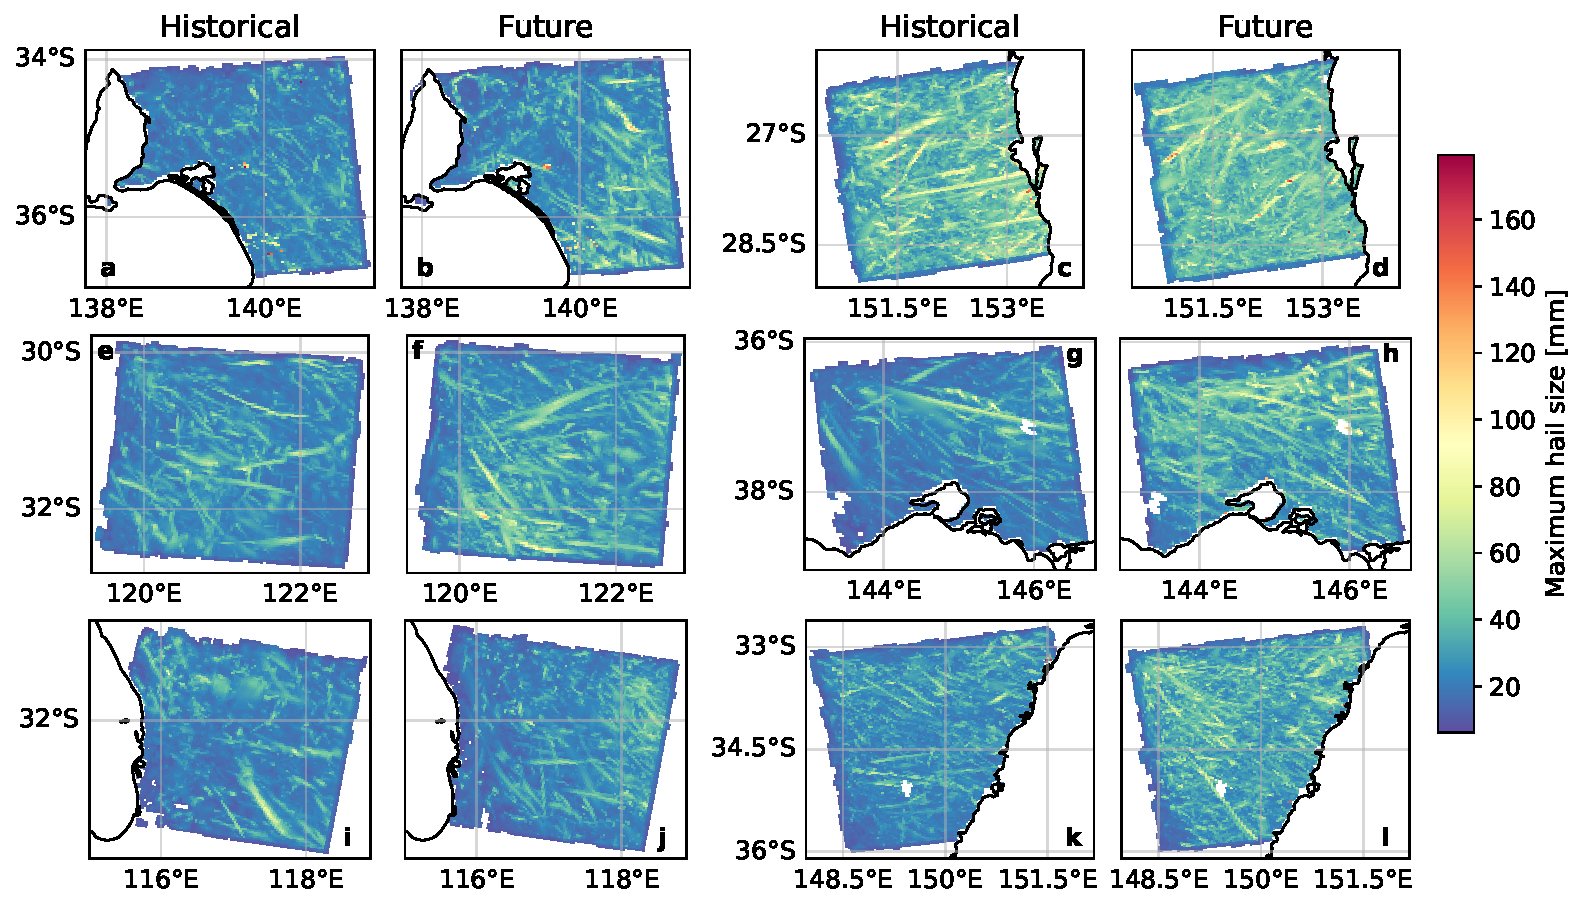
\includegraphics[width=\textwidth]{figures/max_hail_sizes_by_domain}
      \caption{Maximum hail sizes in historical and future climates, for Adelaide (a, b), Brisbane (c, d), Goldfields (Kalgoorlie) (e, f), Melbourne (g, h), Perth (i, j) and Sydney/Canberra (k, l) domains.}
      \label{fig:max_hail_sizes_by_domain}
\end{figure}

\subsection{Changes in frequency of hail}

Table \ref{tab:frequency} shows changes in the frequency of hail days across the six study domains. There are significant increases in hail frequency in the Sydney/Canberra and Brisbane domains, with a 29\% increase in seasonal hail days in the Sydney/Canberra region. There are small non-significant frequency decreases in Adelaide, the Goldfields (Kalgoorlie) and Melbourne domains, and an indication of an increase in seasonal hail days in the Perth region, albeit not statistically significant. The variability in seasonal hail days is similar between epochs.

\begin{table}[!ht]
      \centering
      \caption{Mean and standard deviation of seasonal hail days in the historic and future simulations, and relative future changes with 95\% confidence interval according to Welch's two-sample t-test, per domain. Statistical significance of the change calculated by Welch's two-sample t-test is indicated by $\ast{}$ for a 90\% confidence level ($p < 0.1$) and $\ast{}\!\ast{}$ for a 95\% confidence level ($p < 0.05$).}
      \label{tab:frequency}  
      \begin{tabular}{lrrr@{}l@{}r}
            \hline
            Domain & Historic days & Future days & \multicolumn{3}{r}{Future change} \\ 
            \hline
Adelaide  & 8.7 $\pm$ 4.2 & 8.35 $\pm$ 4.9 & -4\% & $$ & (-38\% to 30\%) \\Brisbane  & 32.95 $\pm$ 8.3 & 37.8 $\pm$ 8.8 & 15\% & $\,\ast{}$ & (-2\% to 31\%) \\Kalgoorlie  & 10 $\pm$ 6 & 9.8 $\pm$ 5.2 & -2\% & $$ & (-38\% to 34\%) \\Melbourne  & 11.7 $\pm$ 5.9 & 11.5 $\pm$ 7.1 & -2\% & $$ & (-37\% to 34\%) \\Perth  & 6.8 $\pm$ 4.9 & 7.55 $\pm$ 4.9 & 11\% & $$ & (-35\% to 57\%) \\Sydney/Canberra  & 24.3 $\pm$ 9.4 & 31.4 $\pm$ 9 & 29\% & $\,\ast{}\!\ast{}$ & (5\% to 53\%) \\
            \hline 
       \end{tabular}
\end{table}

\subsection{Extreme value analysis}

\subsubsection{GEV goodness of fit}

GEV models were fitted to time series of daily maximum hail sizes and 10 m wind speeds at hail hours (Supporting Information Figures \ref{SM-fig:timeseries_hail} and \ref{SM-fig:timeseries_wind}). QQ plots for hail size show acceptable agreement with some model overestimation of high quantiles (Supporting Information Figure \ref{SM-fig:qq_hail}), while QQ plots for wind speed at hail hours show excellent agreement between modelled and empirical quantiles (Supporting Information Figure \ref{SM-fig:qq_wind}). In all cases where the model was compared to empirical values, either all or the bulk of KS test $p$ values were above the 0.05 level, indicating that the null hypothesis that the two samples are drawn from the same distribution can not be rejected (Supporting Material Figure \ref{SM-fig:ks_pvals}). The QQ plot and KS test results show that the GEV models have sufficient goodness of fit for the analyses here. 

\subsubsection{Significance of changes}

Having determined that the GEV fits to empirical data are valid, we now consider whether the fitted models show any significant difference between the historical and future epochs. Figure \ref{fig:gev_parameters} shows the fitted parameters and their confidence intervals for all the GEV models used in this study. The models fitted for the Melbourne and Sydney/Canberra domains both show significant differences between epochs in the location or scale parameters for both hail size and wind at hail hours, whereas the models for the other domains have parameters with overlapping confidence intervals. These results are further supported by the $p$ value distributions from KS tests when historical models are compared to future models (Supporting Information Figure \ref{SM-fig:ks_pvals}). The null hypothesis that the samples are drawn from the same distribution can be rejected for the Melbourne and Sydney/Canberra domains for both maximum hail size and maximum wind speed at hail hours, and for the Perth domain for wind only. To be conservative, we conclude that the changes in maxima between epochs are significant in the Melbourne and Sydney/Canberra domains, but not significant in the other domains.

\begin{figure}[!ht]
      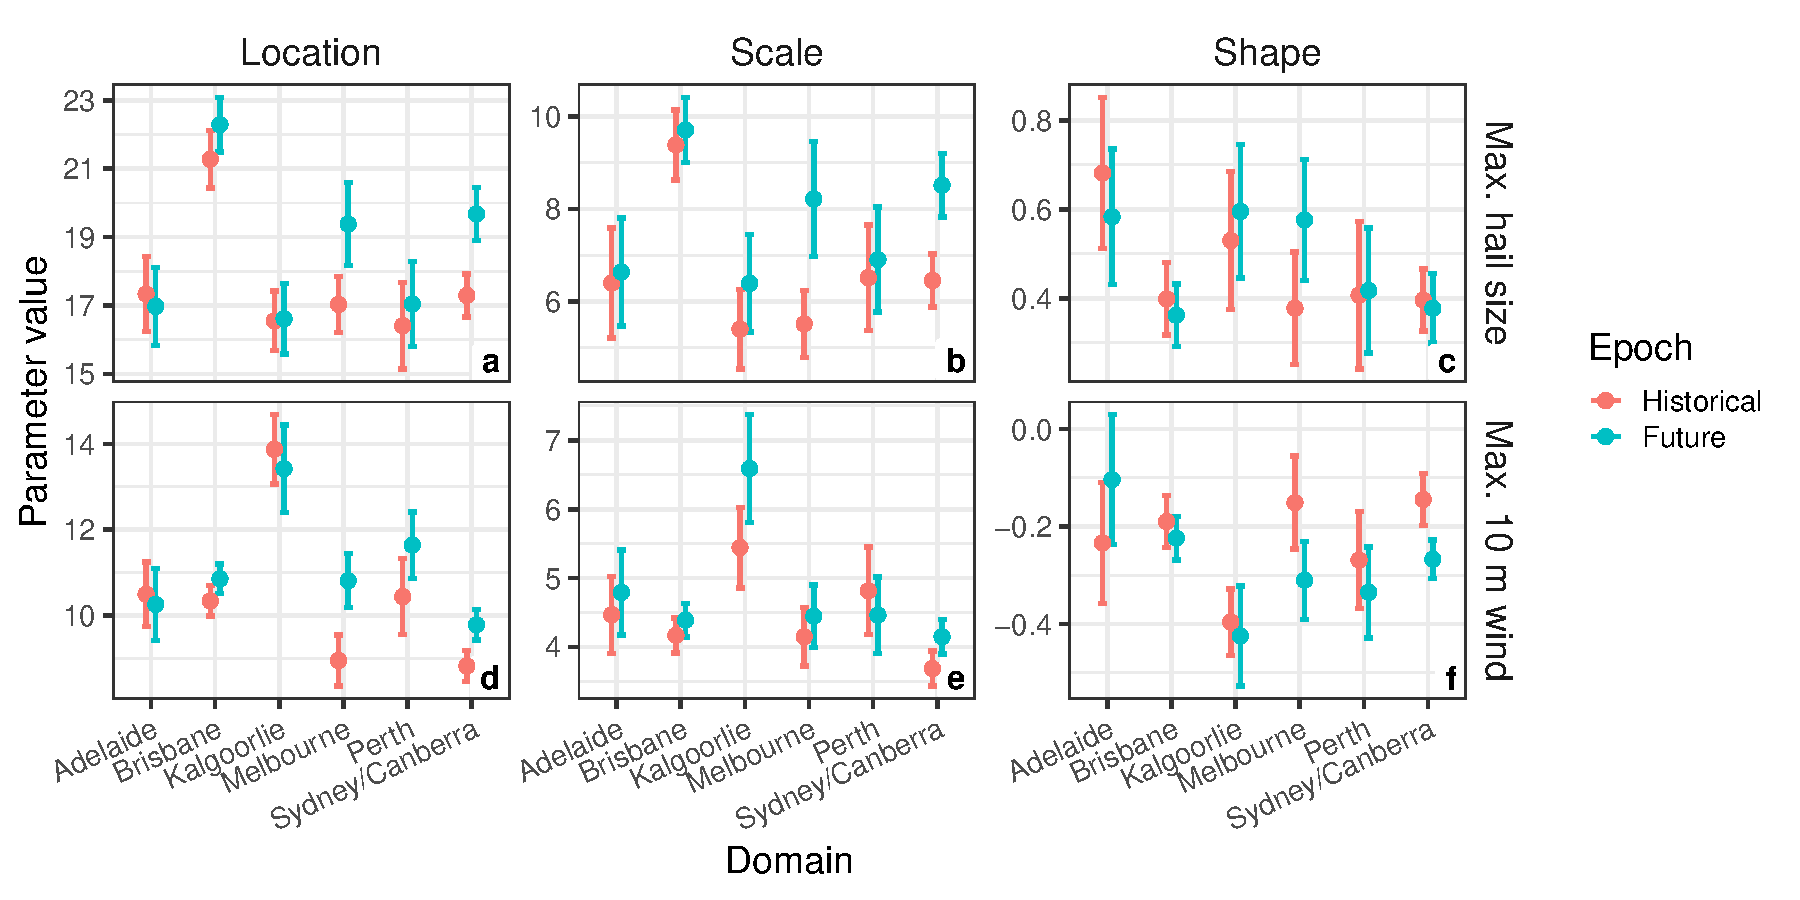
\includegraphics[width=\textwidth]{figures/fit_params}
      \caption{Location (a, d), scale (b, e), and shape (c, f) parameters for fitted GEV distributions for maximum hail size (a--c) and 10 m wind at hail hours (d--f). Parameter values are shown as a point and whiskers show 95\% confidence intervals.}
      \label{fig:gev_parameters}
\end{figure}

\subsubsection{Return periods}

Figure \ref{fig:return_periods_probs_hail} shows return period curves for maximum hail size and maximum wind speed at hail hours. Because our analysis is limited to hail days, the return periods are in number of hail days, not overall days. It is not uncommon for return period models based on the GEV family to produce non-physical extreme values such as the extremely large hail sizes predicted for large return periods here \cite[p. 66]{Coles_2001}. We take the advice of \citeA{Coles_2001} and interpret the results here based on the shorter return periods, thus keeping physical principles in mind. In Melbourne and Sydney/Canberra, the two domains with significant changes, there are increases in the maximum expected hail size for return periods longer than about three hail days, with the largest increase in the Melbourne region where the return period for 100 mm hail is reduced from more than 100 hail days to about 30 hail days. In both domains with significant changes the return period for lighter winds (less than about 18 m s$^{-1}$) is markedly shorter in the future scenario, but the return period for very strong winds is longer in the warmer scenario. For the other domains, with non-significant differences in GEV distributions, the most notable changes are a decrease in strong wind return periods for Adelaide and Goldfields (Kalgoorlie) regions and light wind return periods in the Perth region.

\begin{figure}[!ht]
      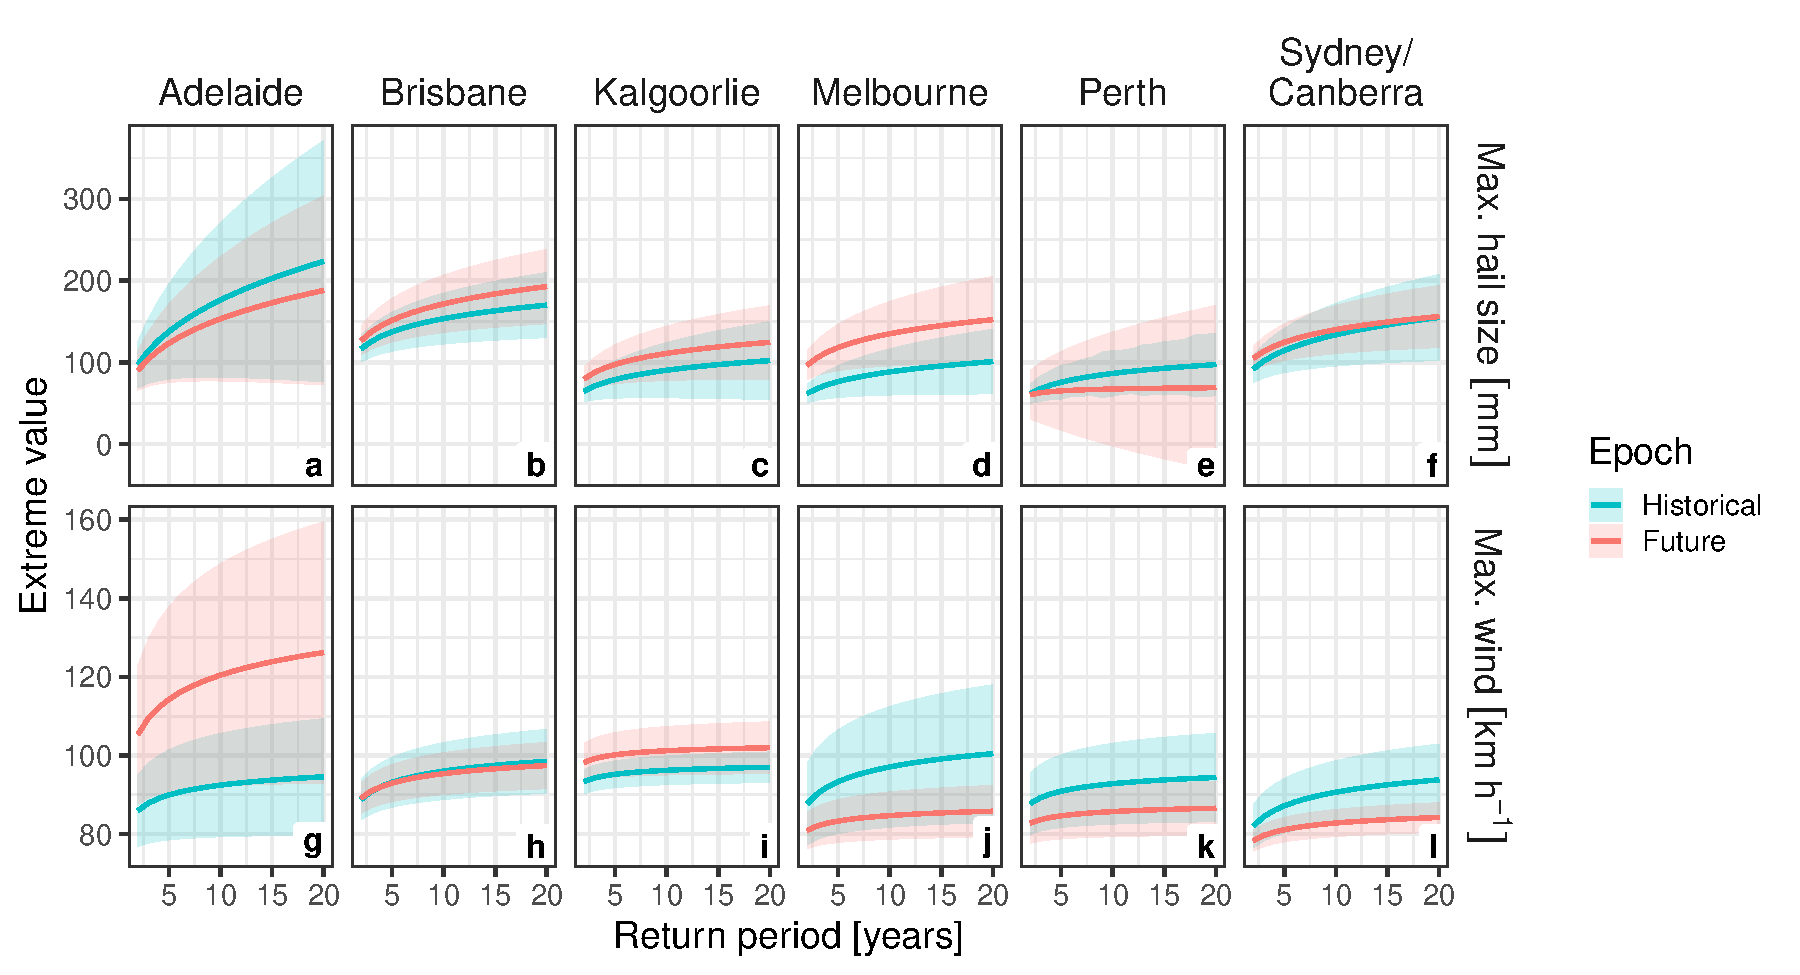
\includegraphics[width=\textwidth]{figures/return_periods}
      \caption{Return period plots for maximum hail size (a--f) and maximum wind at hail hours (g--l) for the domains of Adelaide (a, g), Brisbane (b, h), Goldfields (Kalgoorlie) (c, i), Melbourne (d, j), Perth (e, k), and Sydney/Canberra (f, l).}
      \label{fig:return_periods_probs_hail}
\end{figure}

\subsubsection{Probability of exceeding damaging thresholds}



% <<hailProbResultsSydCan, echo=FALSE, include=TRUE, results="asis">>=
% scSevereHist = round(filter(hail_probs, domain == "Sydney + Canberra", diam==20, epoch=="historical")$p, 0)
% scSevereFut = round(filter(hail_probs, domain == "Sydney + Canberra", diam==20, epoch=="ssp245")$p, 0)
% scGiantHist = round(filter(hail_probs, domain == "Sydney + Canberra", diam==50, epoch=="historical")$p, 0)
% scGiantFut = round(filter(hail_probs, domain == "Sydney + Canberra", diam==50, epoch=="ssp245")$p, 0)
% sc100Hist = round(filter(hail_probs, domain == "Sydney + Canberra", diam==100, epoch=="historical")$p, 0)
% sc100Fut = round(filter(hail_probs, domain == "Sydney + Canberra", diam==100, epoch=="ssp245")$p, 0)

% # Check claims in text.
% if (scSevereHist > scSevereFut) {
%       cat("\\todo{Sydney severe hail does not increase.}")
% }
% if (sc100Hist > sc100Fut) {
%       cat("\\todo{Sydney 100 mm hail does not increase.}")
% }
% @

% <<windProbResultsMelb, echo=FALSE, include=TRUE, results="asis">>=
% melbWindHist = round(filter(wind_probs, domain == "Melbourne", epoch=="historical")$p, 3)
% melbWindFut = round(filter(wind_probs, domain == "Melbourne", epoch=="ssp245")$p, 3)
% scWindHist = round(filter(wind_probs, domain == "Sydney + Canberra", epoch=="historical")$p, 3)
% scWindFut = round(filter(wind_probs, domain == "Sydney + Canberra", epoch=="ssp245")$p, 3)

% # Check statements in text.
% if (any(scWindHist > 0.1) || any(melbWindHist > 0.1)) {
%       cat("\\noindent\\todo{Hist wind probs are $>$ 0.1.}\\\\")
% }
% if (any(melbWindFut != 0) || any(scWindFut != 0)) {
%       cat("\\noindent\\todo{Future wind probabilities are not zero.}")
% } 
% @

Figure \ref{fig:thresholds} shows the probability of a hail day producing various damaging hail and wind thresholds at hail hours (numerical results are shown in Supporting Information Table \ref{SM-tab:exceedence_probs}), comparing historical to future epochs. For hail we examine the probability of a hail day producing severe (20 mm), giant (50 mm), and 100 mm hail, while for wind we examine 80 and 100 km h$^{-1}$ as damaging thresholds. In the Melbourne domain for any given hail day, the probability of severe hail jumps from $\sim$46\% in the historical epoch to $\sim$61\% in the future scenario, while giant hail probability roughly triples (from $\sim$4\% to $\sim$13\%), and 100 mm hail is more than 5 times more likely (from $\sim$1\% to $\sim$4\%) in the future epoch. In the Sydney/Canberra domain, any given hail day has a probability of severe hail of $\sim$49\% in the historical epoch which increases to $\sim$62\% in the future scenario, while giant hail probability ($\sim$6\% to $\sim$10\%) and 100 mm hail probability ($\sim$1\% to $\sim$2\%) both come close to doubling in the future epoch. Other non-significant increases in severe hail probability are shown for Brisbane, Perth, and Goldfields (Kalgoorlie) areas, with non-significant decreases in the Adelaide region, and the Goldfields region shows a non-significant increase also for giant hail probability. In Melbourne and Sydney/Canberra, the domains with significant differences, the probability of damaging winds at hail hours on a hail day decreases by about half for 80 km h$^{-1}$ wind speed at hail hours. Non-significant changes include an increase in the probability of 80 km h$^{-1}$ wind speed at hail hours in the Goldfields (Kalgoorlie) region (from $\sim$9\% to $\sim$13\%) and Adelaide domain (from $\sim$2\% to $\sim$5\%), and for 100 km h$^{-1}$ winds at hail hours for the Adelaide region (from $\sim$0\% to $\sim$1\%).  Other than for Adelaide, the probability of hail days producing 100 km h$^{-1}$ wind speed at hail hours is close to zero in all domains across both epochs. 

\begin{figure}[!ht]
      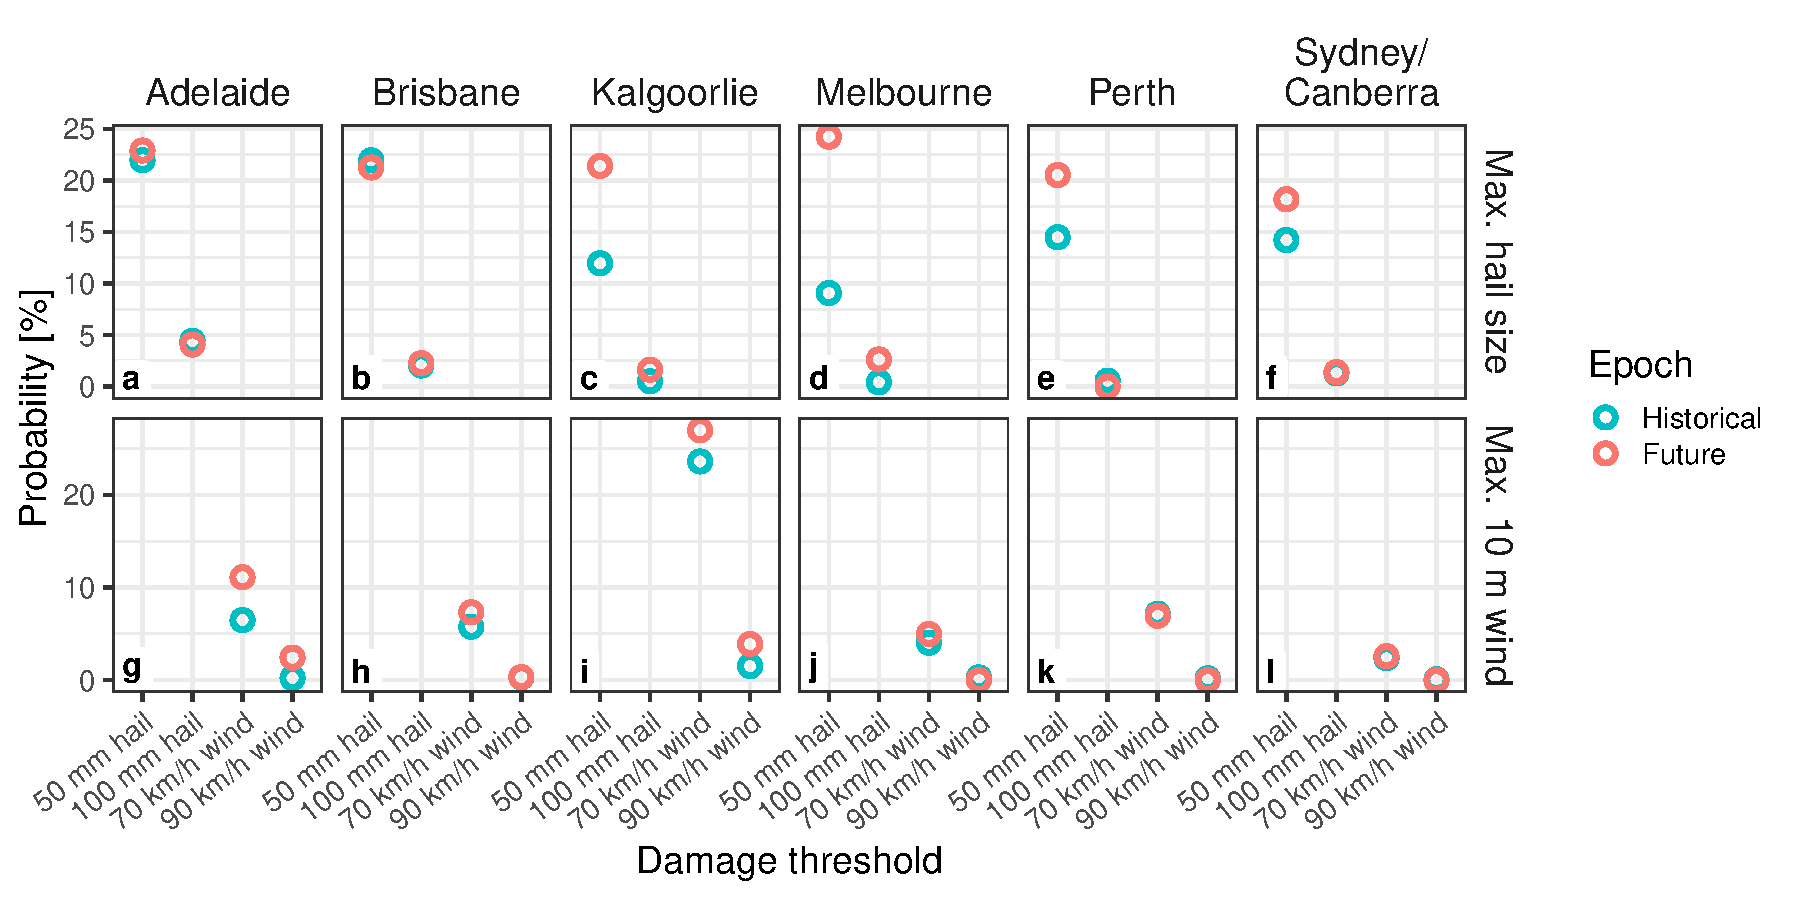
\includegraphics[width=\textwidth]{figures/threshold_probs}
      \caption{Changes in the probability of exceeding thresholds on hail size (a--f), and 10 m wind speed at hail hours (g--l), on any given hail day, for the domains of Adelaide (a, g), Brisbane (b, h), Goldfields (Kalgoorlie) (c, i), Melbourne (d, j), Perth (e, k), and Sydney/Canberra (f, l).}
      \label{fig:thresholds}
\end{figure}

\subsection{Changes in relevant atmospheric properties}

\begin{table}[h!]
      \caption{Projected relative changes in mean convective available potential energy (CAPE), convective inhibition (CIN), freezing-level height (FLH), hail size, lifted index (LI), lapse rate from 700 to 500 hPa (LR), bulk vertical wind shear from 0-6 km (S06), temperature at 500 hPa (T500), and 10 m wind at hail times (Wind), by domain.  Statistical significance of the difference between historical and future seasonal mean values, calculated using Welch's two-sample t-test, is shown by $\ast{}$ for the 90\% confidence level, $\ast{}\!\ast{}$ for the 95\% confidence level, and $\ast{}\!\ast{}\!\!\ast{}$ for the 99\% confidence level. Bracketed ranges show the 95\% confidence interval on the changes.}
      \centering
      \begin{tabular}{lr@{}l@{}rr@{}l@{}rr@{}l@{}r}
            \hline
& \multicolumn{3}{c}{Adelaide} & \multicolumn{3}{c}{Brisbane} & \multicolumn{3}{c}{Kalgoorlie} \\ 
%%%%%%%%%%%%%%%%%%%
\hline
CAPE  & 23\% & $\ast{}$ & (-2\% to 49\%) & 9\% & $\ast{}\!\ast{}$ & (2\% to 15\%) & 11\% & $$ & (-8\% to 29\%) \\
CIN  & -22\% & $\ast{}\!\ast{}$ & (-40\% to -4\%) & -8\% & $\ast{}\!\ast{}\!\!\ast{}$ & (-14\% to -2\%) & -13\% & $\ast{}\!\ast{}$ & (-25\% to -1\%) \\
FLH  & 9\% & $\ast{}\!\ast{}\!\!\ast{}$ & (7\% to 11\%) & 9\% & $\ast{}\!\ast{}\!\!\ast{}$ & (8\% to 10\%) & 9\% & $\ast{}\!\ast{}\!\!\ast{}$ & (6\% to 11\%) \\
Hail size  & 0\% & $$ & (-4\% to 3\%) & 4\% & $\ast{}\!\ast{}\!\!\ast{}$ & (2\% to 5\%) & 0\% & $$ & (-3\% to 4\%) \\
LI  & -41\% & $$ & (-146\% to 65\%) & -8\% & $\ast{}\!\ast{}$ & (-16\% to 0\%) & 77\% & $\ast{}$ & (-7\% to 161\%) \\
LR  & -1\% & $$ & (-3\% to 1\%) & 2\% & $\ast{}\!\ast{}\!\!\ast{}$ & (1\% to 3\%) & -1\% & $$ & (-2\% to 1\%) \\
MLH  & 8\% & $\ast{}\!\ast{}\!\!\ast{}$ & (6\% to 10\%) & 9\% & $\ast{}\!\ast{}\!\!\ast{}$ & (8\% to 10\%) & 9\% & $\ast{}\!\ast{}\!\!\ast{}$ & (6\% to 11\%) \\
S06  & -1\% & $$ & (-9\% to 7\%) & -4\% & $\ast{}\!\ast{}$ & (-7\% to 0\%) & 5\% & $\ast{}$ & (-1\% to 11\%) \\
T500  & 1\% & $\ast{}\!\ast{}\!\!\ast{}$ & (1\% to 1\%) & 1\% & $\ast{}\!\ast{}\!\!\ast{}$ & (1\% to 1\%) & 1\% & $\ast{}\!\ast{}\!\!\ast{}$ & (1\% to 1\%) \\
Wind  & -1\% & $$ & (-7\% to 5\%) & 2\% & $$ & (-1\% to 4\%) & -2\% & $$ & (-7\% to 3\%) \\
\hline 
%%%%%%%%%%%%%%%%%%%
& \multicolumn{3}{c}{Melbourne} & \multicolumn{3}{c}{Perth} & \multicolumn{3}{c}{Sydney/Canberra} \\
%%%%%%%%%%%%%%%%%%%
\hline
CAPE  & 29\% & $\ast{}\!\ast{}\!\!\ast{}$ & (14\% to 44\%) & 14\% & $$ & (-11\% to 38\%) & 25\% & $\ast{}\!\ast{}\!\!\ast{}$ & (16\% to 34\%) \\
CIN  & -23\% & $\ast{}\!\ast{}\!\!\ast{}$ & (-36\% to -10\%) & -7\% & $$ & (-21\% to 6\%) & -15\% & $\ast{}\!\ast{}\!\!\ast{}$ & (-23\% to -7\%) \\
FLH  & 10\% & $\ast{}\!\ast{}\!\!\ast{}$ & (8\% to 12\%) & 8\% & $\ast{}\!\ast{}\!\!\ast{}$ & (4\% to 11\%) & 9\% & $\ast{}\!\ast{}\!\!\ast{}$ & (8\% to 10\%) \\
Hail size  & 4\% & $\ast{}\!\ast{}$ & (1\% to 7\%) & 1\% & $$ & (-3\% to 6\%) & 4\% & $\ast{}\!\ast{}\!\!\ast{}$ & (2\% to 6\%) \\
LI  & -13\% & $$ & (-77\% to 50\%) & 12\% & $$ & (-72\% to 96\%) & -21\% & $$ & (-48\% to 6\%) \\
LR  & 1\% & $$ & (0\% to 3\%) & 1\% & $$ & (-2\% to 3\%) & 2\% & $\ast{}\!\ast{}\!\!\ast{}$ & (1\% to 3\%) \\
MLH  & 10\% & $\ast{}\!\ast{}\!\!\ast{}$ & (8\% to 12\%) & 7\% & $\ast{}\!\ast{}\!\!\ast{}$ & (4\% to 10\%) & 9\% & $\ast{}\!\ast{}\!\!\ast{}$ & (7\% to 10\%) \\
S06  & 6\% & $$ & (-2\% to 13\%) & -2\% & $$ & (-10\% to 6\%) & -1\% & $$ & (-6\% to 3\%) \\
T500  & 1\% & $\ast{}\!\ast{}\!\!\ast{}$ & (1\% to 1\%) & 1\% & $\ast{}\!\ast{}\!\!\ast{}$ & (0\% to 1\%) & 1\% & $\ast{}\!\ast{}\!\!\ast{}$ & (1\% to 1\%) \\
Wind  & 3\% & $$ & (-2\% to 8\%) & 9\% & $\ast{}\!\ast{}\!\!\ast{}$ & (3\% to 15\%) & 3\% & $\ast{}$ & (0\% to 6\%) \\
\hline
%%%%%%%%%%%%%%%%%%%
            \end{tabular}
\end{table}

\subsection{Region correlations}

\section{Conclusions}

\begin{itemize}
      \item \todo{Caution that hail is max size per hour and wind is hourly instantaneous wind}.
\end{itemize}

\section*{Open Research Section}

Boundary condition data are available at \citeA{Xu_code_data_2021}.

% This section MUST contain a statement that describes where the data supporting
% the conclusions can be obtained. Data cannot be listed as ''Available from
% authors'' or stored solely in supporting information. Citations to archived
% data should be included in your reference list. Wiley will publish it as a
% separate section on the paper’s page. Examples and complete information are
% here: https://www.agu.org/Publish with AGU/Publish/Author Resources/Data for
% Authors

\acknowledgments

Since March 2024, THR's position at UNSW Sydney has been supported by QBE Insurance. This research was undertaken with the assistance of resources from the National Computational Infrastructure (NCI Australia), an NCRIS enabled capability supported by the Australian Government. We thank Simon Tett for useful discussions on extreme value techniques.

%% Include references from supporting information.
\nocite{Milbrandt_JAS_2021}
 \nocite{Zhang_JC_2017}
 \nocite{Iacono_JGRA_2008}
 \nocite{Hong_MWR_2006}
 \nocite{Jimenez_MWR_2012}
 \nocite{Niu_JGRA_2011}


\bibliography{library}

\end{document}
